\documentclass{article}
\usepackage[utf8]{inputenc}
\usepackage{graphicx}
\usepackage{mathtools}
\usepackage{amsmath}
\usepackage{hyperref}
\graphicspath{ {./} }

% \title{EulerAlgoGCD}
% \author{Glaives De V�rit�}
% \date{December 2022}
\begin{document}
\begin{flushleft}
\textbf{Algorithm E} (\textit{Extended Euclid's algorithm}). Given two positive integers \textit{m} and \textit{n}, we compute their greatest common divisor \textit{d} and two integers \textit{a} and \textit{b}, such that $am + bn = d$.
\vspace{4mm}
\par \textbf{E1.} [Initialize.] Set $a \gets b \gets 1$, $a \gets b' \gets 0$, $c \gets m$, $d \gets n$.
\vspace{2mm}
\par \textbf{E2.} [Divide.] Let \textit{q} and \textit{r} be the quotient and remainder, respectively, of \textit{c} divided by \textit{d}. (We have $c = qd + r$ and $0\leq r \leq d$.)
\vspace{2mm}
\par \textbf{E3.} [Remainder zero?] If $r = 0$, the algorithm terminates; we have in this case $am + bn = d$ as desired.
\vspace{2mm}
\par \textbf{E4.} [Recycle.] Set $c \gets d$, $d \gets r$, $t \gets a'$, $a' \gets a$, $a \gets t - qa$, $t \gets b'$, $b' \gets b$, $b \gets t - qb$, and go back to E2.
\vspace{3mm}
\par 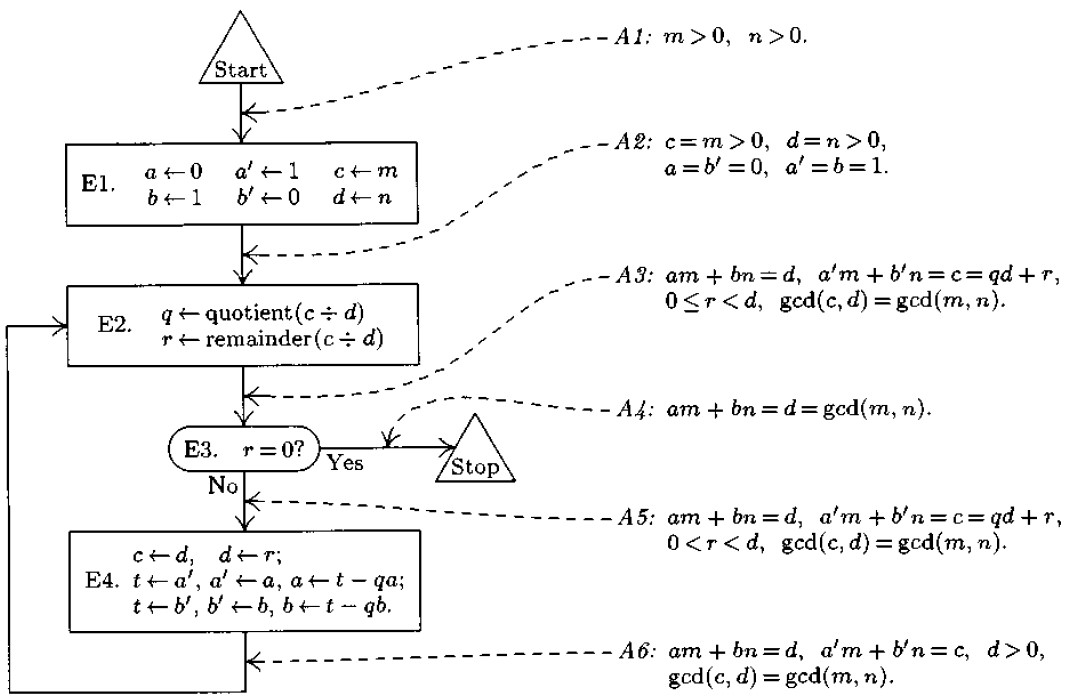
\includegraphics[width=\textwidth]{scheme}
\vspace{3mm}
\par \textbf{My remarks}
\vspace{2mm}
\par Let we found $x_1, y_1 : b \cdot x_1 + (a \bmod b) \cdot y_1 = gcd(a, b)$. Obviously, that $a \bmod {b} = a - \lfloor \dfrac{a}{b} \rfloor \cdot b$. We have:
\par $b \cdot x_1 + (a\bmod {b}) \cdot y_1 = b \cdot x_1 + (a - \lfloor \dfrac {a} {b} \rfloor \cdot b) \cdot y_1 = b \cdot (x_1 - \lfloor \dfrac{a}{b} \rfloor \cdot y_1) + a \cdot y_1 = a \cdot y_1 + b \cdot (x_1 - \lfloor \dfrac{a}{b} \rfloor \cdot y_1)$
\vspace{5mm}
\par \textbf{Resources}
\par \href{https://neerc.ifmo.ru/wiki/index.php?title=%D0%9D%D0%B0%D0%B8%D0%B1%D0%BE%D0%BB%D1%8C%D1%88%D0%B8%D0%B9_%D0%BE%D0%B1%D1%89%D0%B8%D0%B9_%D0%B4%D0%B5%D0%BB%D0%B8%D1%82%D0%B5%D0%BB%D1%8C#:~:text=%D1%8D%D1%84%D1%84%D0%B5%D0%BA%D1%82%D0%B8%D0%B2%D0%B5%D0%BD%2C%20%D1%87%D0%B5%D0%BC%20%D0%BA%D0%BB%D0%B0%D1%81%D1%81%D0%B8%D1%87%D0%B5%D1%81%D0%BA%D0%B8%D0%B9.-,%D0%A0%D0%B0%D1%81%D1%88%D0%B8%D1%80%D0%B5%D0%BD%D0%BD%D1%8B%D0%B9%20%D0%B0%D0%BB%D0%B3%D0%BE%D1%80%D0%B8%D1%82%D0%BC%20%D0%95%D0%B2%D0%BA%D0%BB%D0%B8%D0%B4%D0%B0,-%D0%92%20%D1%81%D1%82%D0%B0%D0%BD%D0%B4%D0%B0%D1%80%D1%82%D0%BD%D0%BE%D0%BC%20%D0%B0%D0%BB%D0%B3%D0%BE%D1%80%D0%B8%D1%82%D0%BC%D0%B5}{ITMO university wiki}

\end{flushleft}

\end{document}

% \maketitle

